\section{Sensor Description}

The sensor used in the experiment consists of a stereo pair of
cameras. The cameras are mounted on an XR4000 robot facing forward,
parallel to the ground plane. The two cameras are aligned parallel to
one another. The stereo baseline is approximately 30 cm. The relative
pose of the cameras were computed by stereo calibration
\cite{zhang1999fcc}. Internal camera parameters were determined by
calibration for each of the cameras \cite{zhang1999fcc}. 

The cameras are capable of capturing colour images at a maximum
resolution of 640x480 at the rate of 30 frames per second with
interlacing, however the recoding system on-board of the robot can
sustain a much lower throughput. The capturing system records only odd
fields (320x480) at an average rate of 11.5 frames per second per
camera.

\begin{figure}[htbp]
  \centering
\subfigure[Original image.]{
  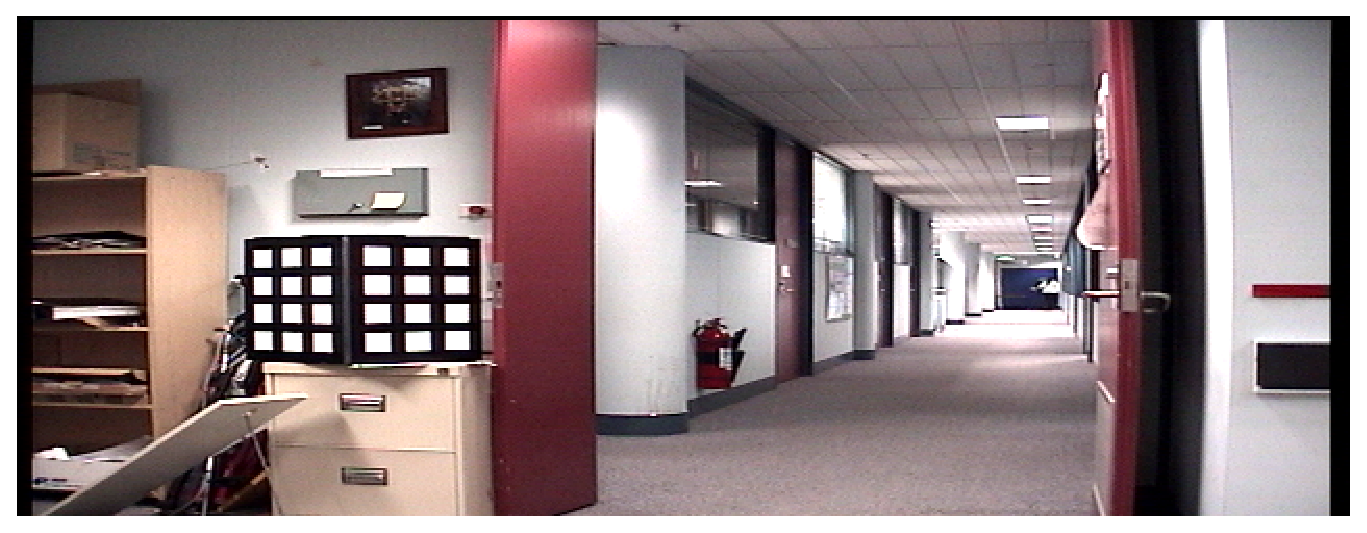
\includegraphics[width=12cm]{Pics/barrel_distortion}
}\\
\subfigure[Corrected image.]{
  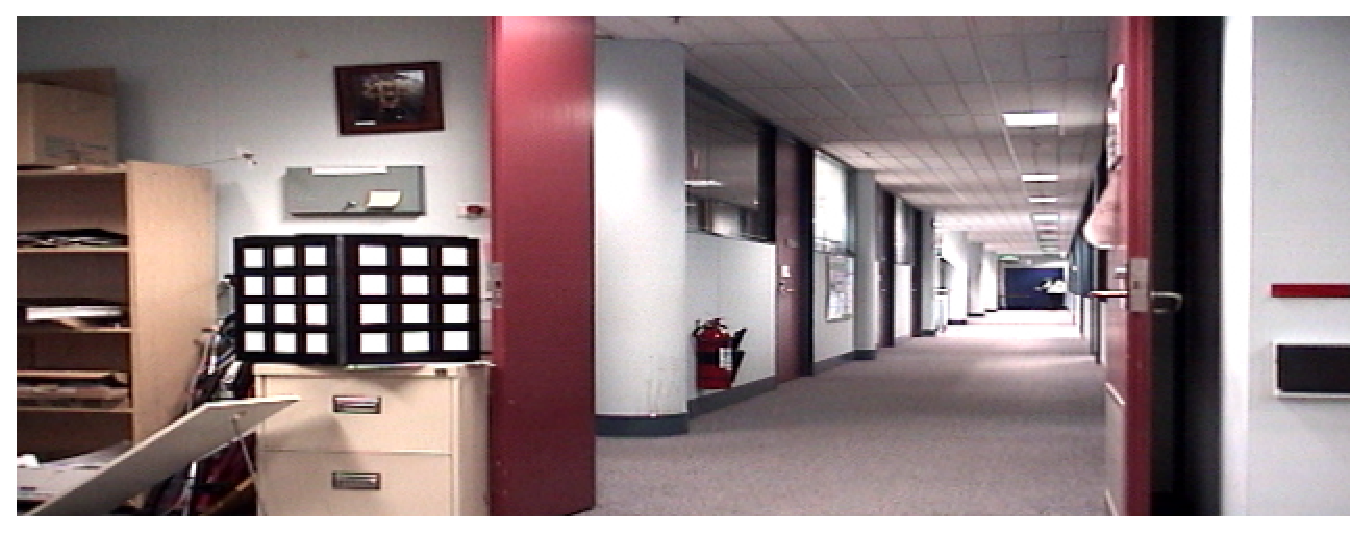
\includegraphics[width=12cm]{Pics/undist_barrel_distortion}
}

  \caption[Barrel distortion]{Effect of barrel distortion.}
  \label{fig:barrel_distortion}
\end{figure}

The cameras used in this experiment have a noticeable barrel
distortion that is corrected in software. The correction is applied
off-line. \refFigure{fig:barrel_distortion} shows an example of
original and corrected images.


\section{Feature Detector: Vertical Edges}

Vertical edges are common in human built environments, and can be
detected fast and reliably. A matched pair of edges in two images
corresponds to a line in world coordinates. A matched pair of vertical
edges corresponds to a vertical line in the world if both
cameras are parallel to the ground plane. A vertical line in a three
dimensional space has only two degrees of freedom and can be defined
completely by a point of intersection with the ground plane. Similarly,
a vertical line in an image plane can be defined completely by a
single parameter: its distance from the left side of an image. A
camera detecting vertical edges is effectively a planar bearing-only
sensor.

By reducing the dimensionality of the sensor from 3d to 2d the
observation model is simplified, which in turn simplifies uncertainty
modelling. Since the robot motion is restricted to the plane, the
vertical dimension can be safely ignored.

The most problematic part of the bearing only SLAM is landmark
creation. One needs at least two bearing observations from different
poses to compute an estimate of landmark location. There are a
number of techniques commonly used \cite{bearing_only_slam}. Since the
robot in this experiment has two cameras, the problem of creating a
new landmark is simplified significantly. Having two cameras also
assists in the data association process. 

The first step of the algorithm is the detection of vertical edges in
the left and right images using vertical Sobel edge detector
\cite{Hartley2004}. To make feature detection more robust, short edges
are discarded as these are more likely to be spurious. Edges that are
only few pixels apart are also removed at this stage.

In the second step correspondances between edges in the left and right
images are established. The cameras on the robot are aligned to be
parallel, and as a result epipolar lines are along the $x$
axis\cite{Hartley2004}. Normalised cross-correlation is used to
establish initial matches. Matches with correlation higher than a
predefined threshold are accepted. If too many matches ($>5$) are
found for a particular edge, this edge is removed. Edges that had no
correspondence are also removed. For the remaining edges the best
three matches are considered.

It is clearly impossible that two distinct edges in the left image
appear in the same spot in the right image, without one being hidden
by another, in which case the depth of the edges cannot be
determined. The matching process has to consider all pairwise matches
to avoid matching the same edge in one image to several edges in the
other.

One can visualise this problem as a graph: every pair of matched edges
defines a node in the graph. Nodes of the graph that do not share a
common edge in both images are connected. The largest fully connected
subgraph of this graph (commonly referred as ``clique'' or ``maximal
clique'' of a graph) corresponds to the largest set of compatible edge
matches. The problem of finding the clique of a graph is NP complete
\cite{cook1971ctp}, which is intractable for a large set of
features. There are, however, methods that can find an approximate
solution \cite{balas1986fmc,pardalos1994mcp}. The approach adopted in
this work is a simple greedy search algorithm with the follwoing steps:

\begin{enumerate}
\item Sort matches in descending order according to their normalised
  cross-correlation results.
\item Set output set to empty.
\item Take one item from the top of the sorted input set.
\item If compatible with all elements in the output set, add it to the
  output set, else discard.
\item Repeat 3 and 4 until the input set is empty.
\end{enumerate}

The compatibility step in the algorithm above can be implemented to
have a constant time computational complexity. The overall
computational complexity of the algorithm is therefore $O(N \log N)$ -
the complexity of the sort.

\begin{figure}[htbp]
  \centering
  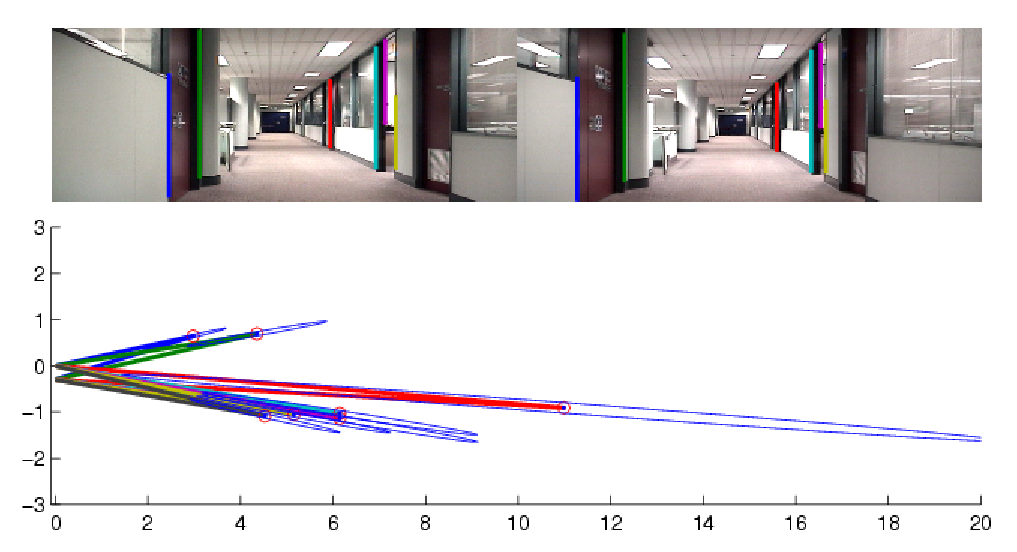
\includegraphics[width=13cm]{Pics/example_edge_detector}
  \caption[Edge Detection Example]{Edge Detection Example: the two
    video frames from the left and right cameras are shown in the
    upper row, the plot below shows location of the edges in the
    sensor centric reference frame and their corresponding
    uncertainties.}
  \label{fig:example_edge_detector}
\end{figure}

An example of vertical edge detection is shown in
\refFigure{fig:example_edge_detector}. Edge correspondences are
indicated by colour: a blue edge in the left corresponds to a blue
edge in the right image, green to green, and so forth. Locations of
the features in the reference frame of the left camera are also
shown. Landmark uncertainty is also shown. Note that cartesian
uncertainty is only used for initialisation of landmarks. Landmark
update equations assume a bearing-only model.

The appearance of a feature provides important information to the
mapping module by assisting in data association. This is especially
usefull in situations when two edges are very close spatially (like
the cyan and magenta edges (edges 4 and 5, counting from the left) in
the \refFigure{fig:example_edge_detector}).

Since vertical edges are generally uniform along the vertical
dimension, the edge template can be ``compressed'' by computing the
average intensity along the vertical dimension. The experiments
presented use a template width of 7 pixels. Since all three colours
per pixel are considered, each template is represented by 21 integer
values. Using only 7 pixels per feature (21 values) greatly reduces
computational effort for template matching. Templates are also
normalised to have zero mean, making correlation computation fast (21
multiplications and 20 additions in this case). Normalisation also
makes template matching less sensitive to variations in lightning
conditions.

\subsection{Sensor Uncertainty}

There are several sources of uncertainty in the sensor. Some
uncertainty comes from the fact that camera calibration is not
perfect. The camera focal length $F$ and principal point $C$ are not
known exactly and might also vary slightly during the experiment. A
second source of uncertainty is the feature extraction mechanism. As
point of view changes, an edge might be detected on a slightly
different part of a physical object. Furthermore, discretisation
errors might add noise as well.

Bearing observation is computed from the column pixel $p$ using the
following equation

$$
z = f([p,C,F]^T) = \frac{p - C}{F}.
$$

The Jacobian of $f$ with respect to $[p,C,F]^T$ ,$\bigtriangledown f$, is used to compute the
approximate Gaussian uncertainty of $z$ from the uncertainties of
$[p,C,F]^T$:

$$
\bigtriangledown f = \left[ 
\frac{1}{F},
\frac{1}{-F},
\frac{-p + C}{F^2}
\right].
$$

The uncertainty of the bearing is then 

$$
\sigma^2_z = \bigtriangledown f \left[ \begin{array}{ccc}
      \sigma^2_p & & \\
   &  \sigma^2_C & \\
  & & \sigma^2_F 
\end{array} \right] \bigtriangledown f^T.
$$



\section{Edge Landmarks}

An edge landmark may be treated as a point landmark with some
additional attributes. The extra attributes include the normalised
edge template (7 pixel x 3 colours = 21 values) and a list of all
observations of the landmark.  The normalised average template is used
to aid in data association and also during the map matching when
closing loops. A list of observations is also used during data
association if the result of matching with the average template failed
to produce a definitive answer.

The data structure used to hold the list of observations can be copied
in constant time, so there is no undue computational burden for
keeping this information. Memory requirements however grow as more
observations are collected. It is not absolutely necessary to keep all
this information, as the average template is usually sufficient. The
main motivation for doing so is to allow accurate template matching in
situations where the appearance of the landmark changes significantly
with observation angle.

The goal of keeping templates is to provide a comprehensive
representation of the appearance of the landmark from various view
points. This can be achieved with relatively few templates. It is not
necessary to store all of them. An approach like principal component
analysis \cite{jolliffe2002pca} can be used to find a sufficient set
of templates for a given edge feature. This problem is, however, beyond
the scope of this thesis.

The true landmark state ${\bf x} = \left[x,y \right]^T$ represents its
location in the local reference frame. The camera pose in the local frame
is denoted $x_c,y_c$ and camera orientation is $\theta_c$. For clarity,
define $x'=x-x_c$ and $y'=y-y_c$. Observation $z_k$ and
landmark states are related by the non-linear function $h$, defined by
($v = N(0,\sigma_{v}^2)$ is a measurement noise)

$$
z_k = h({\bf x},v) =
\frac{-x'\sin \theta_c + y' \cos \theta_c }
     {+x'\cos \theta_c + y' \sin \theta_c } + v.
$$

The true state of the landmark is not known, but the estimate of the
landmark state at time $k$, $\hat{\bf x}_k$, is available. The
estimated covariance of the landmark is maintained by the EKF
and is denoted $P_k$. For clarity, define also
$\hat{x_k}'=\hat{x_k}-x_c$ and $\hat{y_k}'=\hat{y_k}-y_c$.

Additionally, define a Jacobian of partial derivatives of $h$ with
respect to the landmark state:

$$
H_{[i,j]} = \frac{\partial h_{[i]}}{\partial {\bf x}_{[j]}}
             \left(\hat{\bf x}_k , 0 \right).
$$

It is equal to

$$
  H = \left[ 
\begin{array}{c}
\frac{-\hat{y_k}'}
{\hat{x_k}'^2 \cos^2 \theta_c + 2\hat{x_k}'\hat{y_k}'\cos\theta_c\sin\theta_c + \hat{y_k}'^2\sin^2  \theta_c }\\
{}\\
\frac{\hat{x_k}'}
{\hat{x_k}'^2 \cos^2 \theta_c + 2\hat{x_k}'\hat{y_k}'\cos\theta_c\sin\theta_c + \hat{y_k}'^2\sin^2 \theta_c }
\end{array}
      \right].
$$

These Jacobians are used by the EKF, and also during data association,
to project landmark uncertainty into the observation space.

The Jacobian of partial derivatives of $h$ with respect
to noise is also needed by the EKF, and in this case it is trivially

$$
V_{[i,j]} = \frac{\partial h_{[i]}}{\partial v_{[j]}}
             \left(\hat{\bf x}_k , 0 \right) = 1.
$$


\subsection{Data Association}

First, all landmarks are projected into the observation space, both
into the left and right camera. Those landmarks that fall outside the
sensor range are discarded. For each observation the most likely
landmark is found using the nearest neighbour search. 

The quality of a match between a landmark and a single bearing
observation is computed using the following:

$$
  {\bf w}_k = \int p(z_k|^z{\bf x}_k)p(^z{\bf x}_k) d^z{\bf x}.
$$

Here $^z{\bf x}_k$ is a landmark projected into the camera plane, and
$p(^z{\bf x_k})$ is approximated to be a Gaussian, EKF style:

$$
p(^z{\bf x}_k) = N(h(\hat{\bf x}_k,0), H P_k H^T).
$$

The term $p(z_k|^z{\bf x}_k)$ represents the measurement uncertainty
and is also a Gaussian distribution $N(z_k ,\sigma^2_{vk})$. Since
both distributions are Gaussians, the integral of their product can be
computed analytically.

Both left and right bearing have to match the landmark. The total
quality of the match is a product of the left and right weights ${\bf
  w}^l_k{\bf w}^r _k$.

Template matching is used to aid data association as a binary pass or
fail operator. Template matching is only performed if the spatial
tests have passed.

Nearest neighbour is the most common approach to data association, due
to its simplicity, however there are some drawbacks to this
method. The fact that observations were extracted from the same video
frame provides an important piece of information - that these
observations are of different physical entities. Nearest neighbour
search discards this information. Different observations from the same
video frame can be assigned to the same landmark.

Ideally the data association process should take all available
information into consideration. One can use the joint compatibility
data association \cite{neira01:_data_assoc_stoch_mappin_using}, or one
might explore the complete set of possible data associations directly
by sampling from the set of all possible data association decisions
\cite{nieto2003}. In this work nearest neighbour search assisted by
template matching proves sufficient, however a better data association
approach is likely to improve the success rate of the existing
approach.


\subsection{Observation Update}

An observation is treated as two independent bearing-only
observations, first left then right. The standard EKF update equations
are applied to update the estimate of the landmark state and its
covariance.

The landmark template is also updated. It is simply an average of all
observation templates. Each landmark maintains a count of the number
of times it has been observed and a sum of all templates. The average
template is computed from the sum by simply dividing by the total
number of observations. After that, the template is normalised such
that the mean is equal to zero and the sum of deviations from the
mean squared is equal to 1. The normalisation is pre-computed to speed up
the computation of normalised cross correlation.


\subsection{Genesis}

When an edge pair does not match any of the existing landmarks in
the map, a new landmark is added to the map. The initial landmark pose
and the corresponding uncertainties are computed from the observations
using the equations described below.

Let $x_r,y_r$ be the location of the right camera with respect to the
left one and $\theta_r$ be the orientation of the right camera
relative to the left one. Let $u_l,u_r$ be the bearing observations
(tangent of the angle) from the left and right cameras
respectively. We then define the observation to be

$$
{\bf z} =  \left[
    \begin{array}{c}
       u_l\\u_r\\x_r\\y_r\\\theta_r
    \end{array}
\right].
$$

The landmark state can be computed from the observation using the
following:

$$
{\bf x} = f\left({\bf z}\right) 
= \left[\begin{array}{c}
\frac{y_r - x_r\tan(\tan^{-1} u_r+\theta_r)}{u_l-\tan(\tan^{-1} u_r+\theta_r) }\\
{}\\
\frac{y_r - x_r\tan(\tan^{-1} u_r+\theta_r)}{u_l-\tan(\tan^{-1} u_r+\theta_r)}u_l
\end{array}
\right].
$$

Assume that the uncertainty of the observation is a Gaussian with
the following block-diagonal covariance matrix:

$$
C_z = \left[
  \begin{array}{ccc}
    \sigma^2_{ul} &             & \\
                & \sigma^2_{ur} & \\
                &             & \Sigma_{xy\theta}
  \end{array}
\right].
$$

Computing the Jacobian of $f$ with respect to each of the
observation elements,

$$
{\bf J}_{[i,j]} = \frac{\partial f_{[i]}}
{\partial z_{[j]}}\left(z \right)
$$

the initial uncertainty of the feature is then:

$$
P = {\bf J} C_z {\bf J}^T.
$$

The landmark template is initialised to that of the observation.

\section{Defining Map Region}

Unlike laser range sensors, vision sensors cannot provide free space
information easily. It is therefore assumed that no free space
information is available. The approach for defining region bundaries
is identical to that used for the Victoria park data set, with an
exception of the size of the initial region and the size of grid
cells, which were set to be smaller.

\section{Results}

Vision data has been collected together with the laser corner data so
that a comparison can be made between vision and laser
experiments. The vision data set was processed with 100 and 300
particles. One hundred runs of the algorithm were taken to judge the
robustness of the algorithm (100 for 100 particles and 100 for 300
particles).
%\subsection{Maps}

Figures~\ref{fig:edge_map_300p} and \ref{fig:edge_map_100p} show the
map produced for one of the runs using 300 and 100 particles
respectively. Local maps are projected into the reference frame of the
first region. 

Vision is a much more challenging sensor than laser. While most of the
runs have produced good map, many runs
failed. Table~\ref{tab:results_vision} lists the success/failure rates
for the experiment.

\begin{table}[ht]
\center
\begin{tabular}{r|c|c|c}
Num. Particles & Consistent & Consistent but improper & Inconsistent\\
\hline
100 & 67 & 1 & 32\\
300 & 71 & 5 & 24\\
\end{tabular}
\caption{Vision indoors: Summary of the experiments.}
\label{tab:results_vision}
\end{table}

Increasing the number of particles makes the algorithm more robust,
but only slightly. Figures~\ref{fig:edge_map_300p_broken} and
\ref{fig:edge_map_300p_borken2} show examples when HTSLAM did not
succeed to build a proper map. \refFigure{fig:edge_odo_all} shows the
paths of all 100 experiments projected into the reference frame of the
first region.

%Refer to the laser results, same data set. 

\begin{figure}[htbp]
  \centering

  \subfigure[Projection of the HTSLAM map in the reference frame of map 1.]{
    \includegraphics[width=15cm]{Pics/edge_map_300p}
  }\\
  \subfigure[Topological path of the robot.]{
    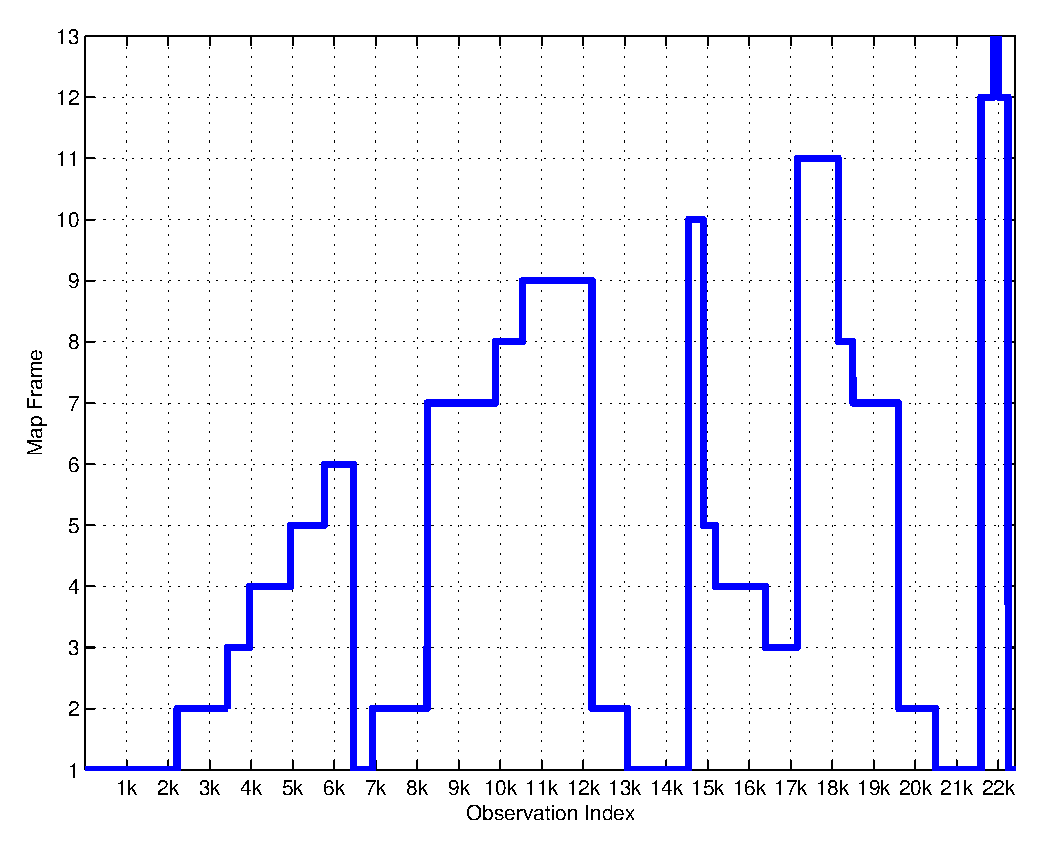
\includegraphics[width=10cm]{Pics/edge_odo_300p}
  }

  \caption{Vision indoors: Map of edges (300 particles/map 52)}
  \label{fig:edge_map_300p}
\end{figure}

\begin{figure}[htbp]
  \centering
  \subfigure[Projection of the HTSLAM map in the reference frame of map 1.]{
    \includegraphics[width=15cm]{Pics/edge_map_100p}
  }
  \subfigure[Topological path of the robot.]{
    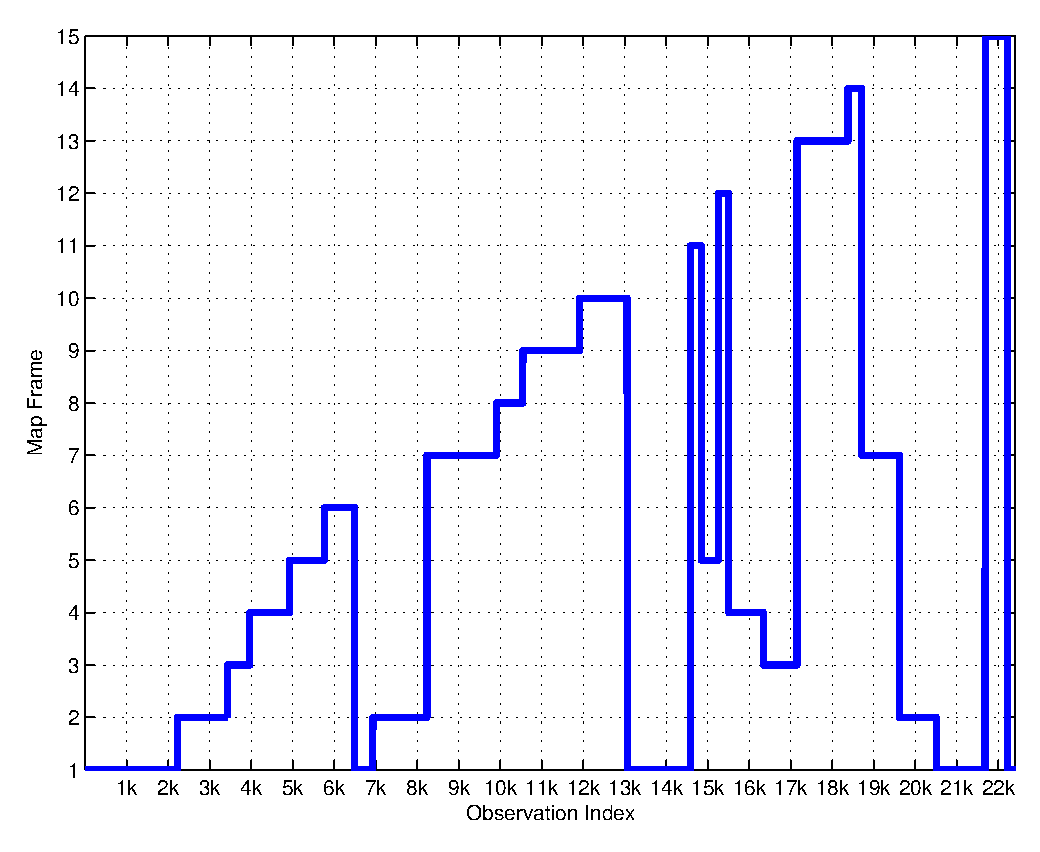
\includegraphics[width=10cm]{Pics/edge_odo_100p}
  }
  \caption{Vision indoors: Map of edges (100 particles/map 89)}
  \label{fig:edge_map_100p}
\end{figure}

\begin{figure}[htbp]
  \centering
  \subfigure[Projection of the HTSLAM map in the reference frame of map 1.]{
    \includegraphics[width=15cm]{Pics/edge_map_300p_broken}
  }
  \subfigure[Topological path of the robot.]{
    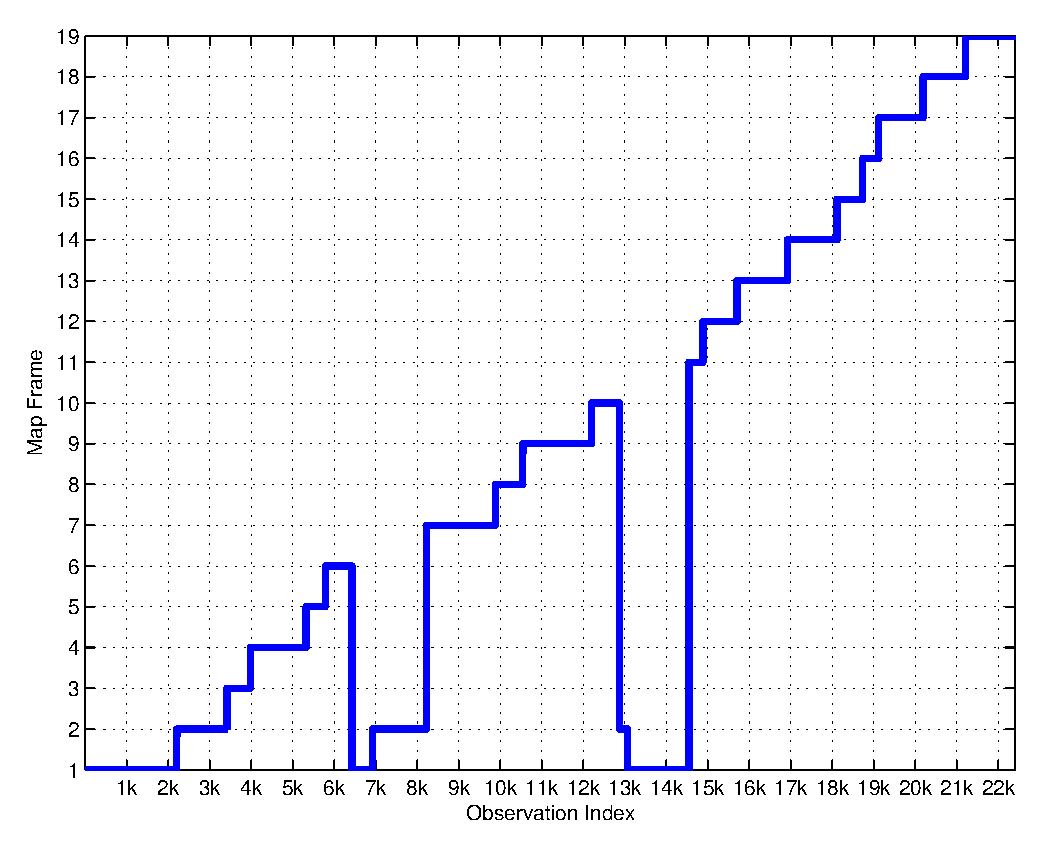
\includegraphics[width=10cm]{Pics/edge_odo_300p_broken}
  }
  \caption{Vision indoors: Jumped out, failed to come back(300 particles/map 40).  Topologically correct, but not ``optimal''}
  \label{fig:edge_map_300p_broken}
\end{figure}

\begin{figure}[htbp]
  \centering
  \subfigure[Projection of the HTSLAM map in the reference frame of map 1.]{
    \includegraphics[width=15cm]{Pics/edge_map_300p_broken2}
  }
  \subfigure[Topological path of the robot.]{
    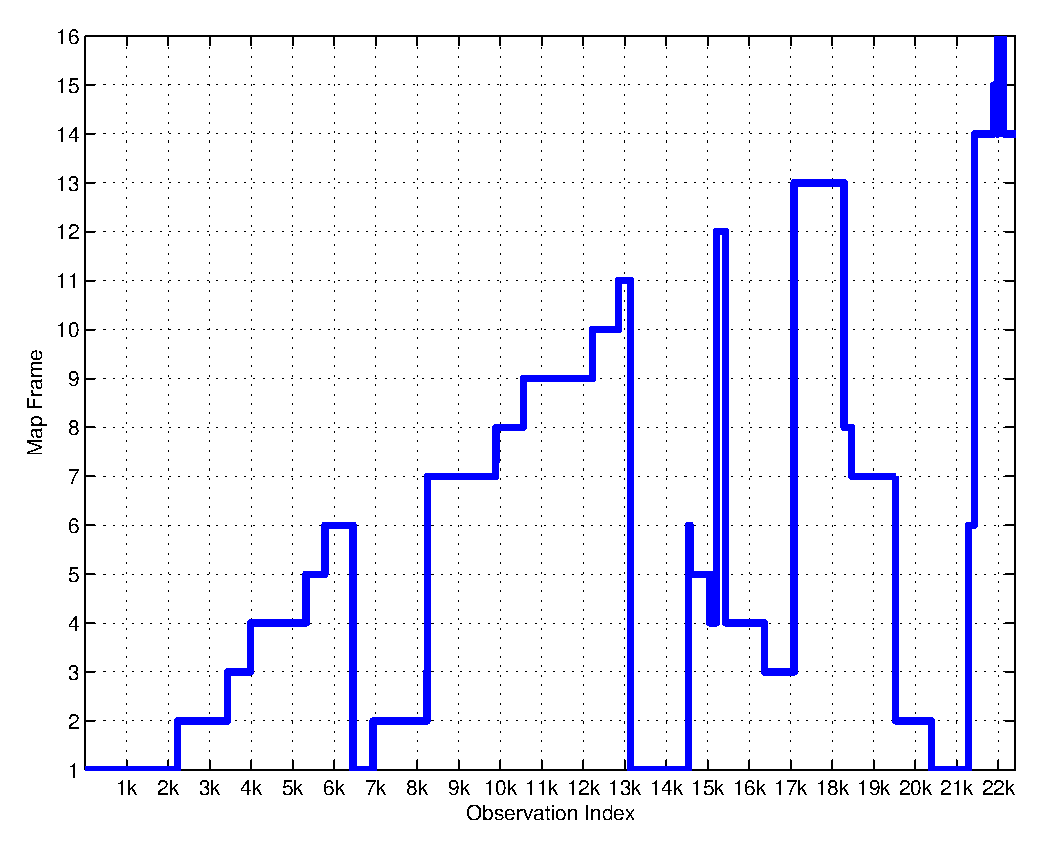
\includegraphics[width=10cm]{Pics/edge_odo_300p_broken2}
  }

  \caption{Vision indoors: Failed transition 7 to 2 (300 particles/map
    18).}
  \label{fig:edge_map_300p_borken2}
\end{figure}

\begin{figure}[htbp]
  \centering
  \subfigure[100 particles]{
    \includegraphics[width=15cm]{Pics/edge_odo_all_100p}
  }
  \subfigure[300 particles]{
    \includegraphics[width=15cm]{Pics/edge_odo_all_300p}
  }
  \caption{Vision indoors: Global Path over 100 test runs.}
  \label{fig:edge_odo_all}
\end{figure}



\subsection{Error Analysis}

There are a number of reasons for a poorer performance of the vision
SLAM when compared to a corner detector in the same environment:

\begin{itemize}
\item Data association is quite challenging with this type of
sensor. 
\item Poor calibration of the sensor.
\item Unmodelled sensor error correlations.
\item Sub-optimal local region assignment
\end{itemize}

Data association is especially difficult when revisiting the region
when travelling in an opposite direction. The appearance of landmarks
can vary significantly when viewed from a different
angle. Furthermore, a very different set of landmarks is visible when
traversing a region in opposite direction. This makes transitions back
into a mapped region from a different direction prone to data
association errors.

Camera provides a rather accurate bearing measurement. As a result the
performance of the sensor is sensitive to calibration errors. The more
accurate your sensor is, the more obvious the impact of biases in the
error model will be.

Another important factor to consider is the effect of unmodelled
correlations between errors in individual observations. All features
detected in the same video frame share common source of uncertainty:
camera calibration parameters. Yet errors are assumed independent for
practical reasons.

As mentioned previously vision and corner data sets were collected
from the same platform at the same time, yet one can see that local
region assignment is significantly different between the two data
sets. In corner based SLAM occupancy grid was used to define a local
region. In the case of vision based experiment no free space
information was available, hence regions were assigned to be of fixed
size. Using free-space information for local region assignment is
advantageous as it partitions the space in a more sensible way. As a
result local region transitions are more reliable.

% LocalWords:  epipolar EKF Jacobians Gaussians IDE Sobel  cyan discretisation
% LocalWords:  HTSLAM odometric odometry
